\documentclass[a4paper,fontset = windows]{ctexbook}
\usepackage{xifthen}
\usepackage{calc}
\usepackage{graphicx}
\usepackage{tikz}
\usepackage[user=teacher]{cexam}

\begin{document}
\chapter{基本排版程序}

\begin{choices}
   1. 这是选择题的题干部分,这部分主要是文字,但是也是有文字的。
   \choice[A] 这是选项A
   \choice[B] 这是选项B
   \choice[C] 这是选项C
   \choice[D] 这是选项D

   2.(2020·陕西省商洛市模拟)如图所示,质量为1 kg的物体与地面间的动摩擦因数$\mu =0.2$,从$ t=0$开始以初速度v0沿水平地面向右滑行,同时受到一个水平向左的恒力$ F=1 N$ 的作用,$ g$取$ 10 m/s^2$,以水平向右为正方向,该物体受到的摩擦力Ff随时间变化的图像是(最大静摩擦力等于滑动摩擦力)
   \choice[P] 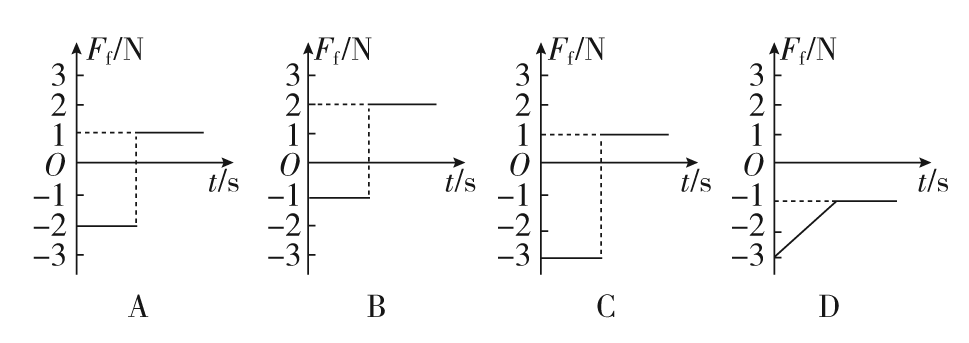
\includegraphics{1.png}

   a.这是答案

\end{choices}

 \begin{blanks}
  1.用 $v-t$ 图像表示小车的运动情况时,以速度$v$ 为\blank{纵轴}、时间 $t$ 为\blank{横轴} 建立直角坐标系,用描点法画出小车的 $v-t$ 图象,图线的 \blank{斜率} 表示加速度的大小,如果 $v-t$ 图象是一条倾斜的直线,说明小车的速度是\blank{均匀变化}的。
 
 a.*
 
 e.此题考察 $v-t$ 图象的意义,通过 $v-t$ 图象识别加速度和判断物体运动特征。
 
 \end{blanks}

 \begin{panduan}
  1.用 $v-t$ 图像表示小车的运动情况时,以速度$v$ 为\blank{纵轴}、时间 $t$ 为\blank{横轴} 建立直角坐标系,用描点法画出小车的 $v-t$ 图象,图线的 \blank{斜率} 表示加速度的大小,如果 $v-t$ 图象是一条倾斜的直线,说明小车的速度是\blank{均匀变化}的。
 
 a.*
 
 e.此题考察 $v-t$ 图象的意义,通过 $v-t$ 图象识别加速度和判断物体运动特征。

 \end{panduan}

\end{document}
